\documentclass[xetex,serif,mathserif]{beamer}

\usepackage{hyperref}
\usepackage{minted}
\usepackage{stmaryrd}
\usepackage{soul}
\usepackage{graphicx}
\usepackage{alltt}
\usepackage{array}
\usepackage{amsmath}
\usepackage{booktabs}
\usepackage{graphicx}

\usepackage[cm-default]{fontspec}
\usepackage{xunicode}
\usepackage{xltxtra}

\usepackage{xcolor}
\usepackage{tikz}
\usetikzlibrary{shapes.geometric, arrows}
\usetikzlibrary{decorations.text}
\usetikzlibrary{shapes,backgrounds}

\setbeamertemplate{navigation symbols}{}
\usecolortheme[RGB={125,17,12}]{structure}
\usefonttheme{serif}
\usefonttheme{structurebold}
\setbeamercolor{description item}{fg=black}

\definecolor{titlered}{rgb}{0.8,0.1,0.1}
\definecolor{white}{rgb}{1.0,1.0,1.0}
\definecolor{cream}{RGB}{225,216,183}

\newenvironment{slide}[1]{\begin{frame}\frametitle{#1}}{\end{frame}}
\newenvironment{fragslide}[1]{\begin{frame}[fragile]\frametitle{#1}}{\end{frame}}
\newenvironment{verbslide}[1]{\begin{frame}[containsverbatim]\frametitle{#1}}{\end{frame}}

\definecolor{highlight}{rgb}{0.8,0.1,0.1}
\definecolor{expr}{rgb}{0.8,0.1,0.1}
\definecolor{cont}{rgb}{0.1,0.2,0.8}
\definecolor{env}{rgb}{0.0,0.0,0.0}

\title{Laurens \\ {\normalsize A Tracing JIT For a Functional Language} }
\author[shortname]{Spenser Bauman \and Cameron Swords}

\institute[shortinst]{
    Indiana University Bloomington, USA
}

\date{Haskell Implementors Workshop -- Lightning Talk\\ August 31st 2015}

\newcommand{\gcol}[2]{\color{#1} #2 \color{black}}
\newcommand{\cek}[3]{\langle \gcol{expr}{#1} , \gcol{env}{#2} , \gcol{cont}{#3} \rangle}

\tikzstyle{racket} = [rectangle, rounded corners, minimum width=3cm, minimum height=1cm,text centered, draw=black, fill=red!60]
\tikzstyle{json} = [rectangle, rounded corners, minimum width=3cm, minimum height=1cm,text centered, draw=black, fill=blue!60]
\tikzstyle{python} = [rectangle, rounded corners, minimum width=3cm, minimum height=1cm,text centered, draw=black, fill=green!60]
\tikzstyle{arrow} = [thick,->,>=stealth]

\def\theFancyVerbLine{%
  \rmfamily\tiny\arabic{FancyVerbLine}%
  {\tikz[remember picture,overlay]\node(minted-\arabic{FancyVerbLine}){};}%
}

\begin{document}

\frame{\titlepage}

\begin{slide}{Background}
    % What is RPython
  \begin{itemize}
    % \item Language+Framework for implementing \emph{dynamic} language interpreters
    % \item Includes a runtime system with language agnostic JIT compiler
    \item RPython includes a tracing JIT for \emph{dynamic} languages
    % \item Includes a runtime system with language agnostic JIT compiler
    % \item The Haskell heap is a dynamic program
    \item Haskell's heap \emph{looks} dynamic during execution
    \item Previous work:

            \vspace*{1em}
            $\begin{array}{r@{}c@{}l}\begin{array}{r}
            \text{Carl Friedrich Bolz} \\
            \text{Even Wiik Thomassen}\\
            \end{array} & \biggr\}  & \text{Implementing Haskell in RPython}\\\\
            \begin{array}{r}\text{Knut Halvor Skrede}\end{array} & \biggr\} & 
            \begin{array}{l@{}}
            \text{Just-In-Time compilation of}\\
            \text{Haskell with PyPy and GHC}
            \end{array}\\\\
            \end{array}$

    \item Both interpret Core, beat GHCi, lose to GHC
  \end{itemize}
\end{slide}

\begin{slide}{What Can We Do?}

  \begin{center}
  Can we \emph{Efficiently} JIT a lazy language?

  \vspace{3em}

  Pycket\footnote{Tomorrow, Session 1} uses an abstract machine with success

  \vspace{3em}

  What would that look like?
  \end{center}
\end{slide}

\begin{slide}{Design - Classical STG}
  \begin{center}
  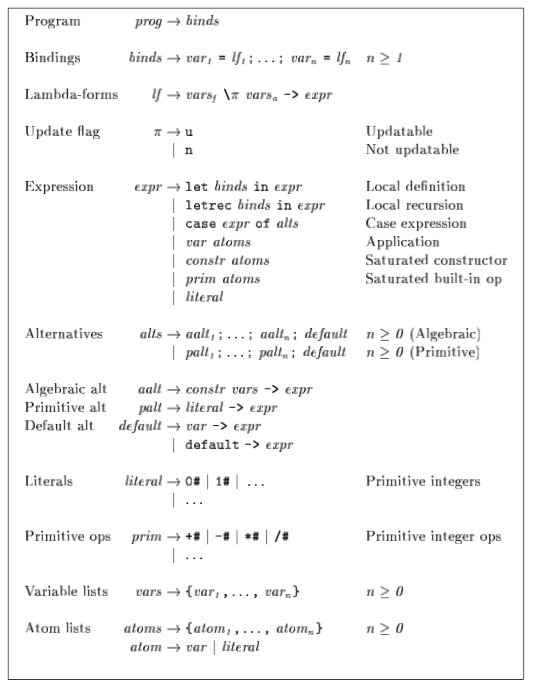
\includegraphics[scale=0.3]{stg-def}
  \end{center}
  % STG Machine
  % Very high level compared to high performance
  % compilers and interpreters
\end{slide}

\begin{frame}[fragile]{Design - Faithful To STG}
  \begin{center}
    \begin{minted}{python}
      def step(self,config):
        code       = config.code
        arg_stack  = config.arg_stack
        ret_stack  = config.ret_stack
        upd_stack  = config.upd_stack
        global_env = config.global_env
        heap       = config.heap
        # Dispatch on |code| ...

      while True:
        config = config.code.step(config)
    \end{minted}
    % Higher-level than compiler
  \end{center}
    % Very high level compared to high performance
    % compilers and interpreters
\end{frame}

\begin{slide}{What Else Can We Do?}


  \begin{center}
  Utilize callgraph model (or suitable variant) from Pycket

  \vspace{3em}
  
  Expose more optimization opportunities for abstract machines (w.r.t STG and generally)

  \vspace{3em}

  Explore tracing in a lazy language\\
  \{fusion, eliding updates, eliminating allocation, ...\}
  \end{center}
\end{slide}



\begin{slide}{Moving Forward}
  \begin{center}
    Refactor implementation into canonical Python

    \vspace{3em}

    Support additional (modern) STG operations

    \vspace{3em}
    
    Construct front-end parser
  \end{center}
    % Validate some claims with Pycket
\end{slide}

\begin{slide}{Conclusion}
    \begin{center}
        \textbf{\sc {\Large Thank You}}

        \vspace{2em}
        Preliminary Implementation\\\href{github.com/cgswords/laurens}{github.com/cgswords/laurens}
    \end{center}
\end{slide}

\end{document}
